Im Versuch wurde die Eingangskennlinie des TTL-NAND-Gatters SN7400 (\textsc{Texas Instruments}) ermittelt.
Dazu wurde der Eingangsstrom bei Veränderung der Gattereingangsspannung (DC)
in einem Bereich von $-1 \, \si{\volt}$ bis $+5 \, \si{\volt}$ gemessen. Die Messergebnisse sind in Tabelle \ref{tab:sn7400ein} zu sehen.

\vspace{\parskip}

\begin{table}[h]
\begin{center}
\begin{tabular}{ll}
\rowcolor{gray0} 
$U_\mathrm{e} / \, \si{\volt}$ & $I_\mathrm{e} / \,\si{\milli\ampere}$ \\
-1                    & -15.9                        \\
-0.9                  & -7.6                         \\
-0.7996               & -3                           \\
-0.7046               & -1.486                       \\
-0.505                & -1.227                       \\
-0.2513               & -1.159                       \\
-0.1048               & -1.12                        \\
-0.0555               & -1.108                       \\
0.0036                & -1.092                       \\
0.0517                & -1.08                        \\
0.1006                & -1.067                       \\
0.2567                & -1.026                       \\
0.5009                & -0.962                       \\
1.0077                & -0.818                       \\
1.5066                & -0.302                       \\
1.5511                & -0.104                       \\
1.7523                & 0.003                        \\
1.6528                & 0                            \\
1.6042                & -0.016                       \\
1.5765                & -0.046                       \\
2.009                 & 0.003                        \\
3.0001                & 0.003                        \\
4                     & 0.003                        \\
4.9833                & 0.004                       
\end{tabular}
\end{center}
\caption{Messergebnisse der Eingangskennlinie des SN7400}
\label{tab:sn7400ein}
\end{table}

Man erkennt einen nichtlinearen Zusammenhang aus der Eingangskennlinie (Abb.
\ref{fig:7400_eingang}). Ab einer Eingangsspannung von etwa $-0.6 \, \si{\volt}$
beginnt der Eingangsstrom stark zu steigen (betragsmäßig). Dies liegt
möglicherweise daran, dass der Basis-Emitter-Übergang des
Multiemittertransistors der TTL-Eingangsstufe immer stärker in Durchlass gerät. Bei einer Spannung von ca. $1.75 \, \si{\volt}$ sättigt sich der Ausgangsstrom.

\begin{figure}[h]
  \begin{center}
    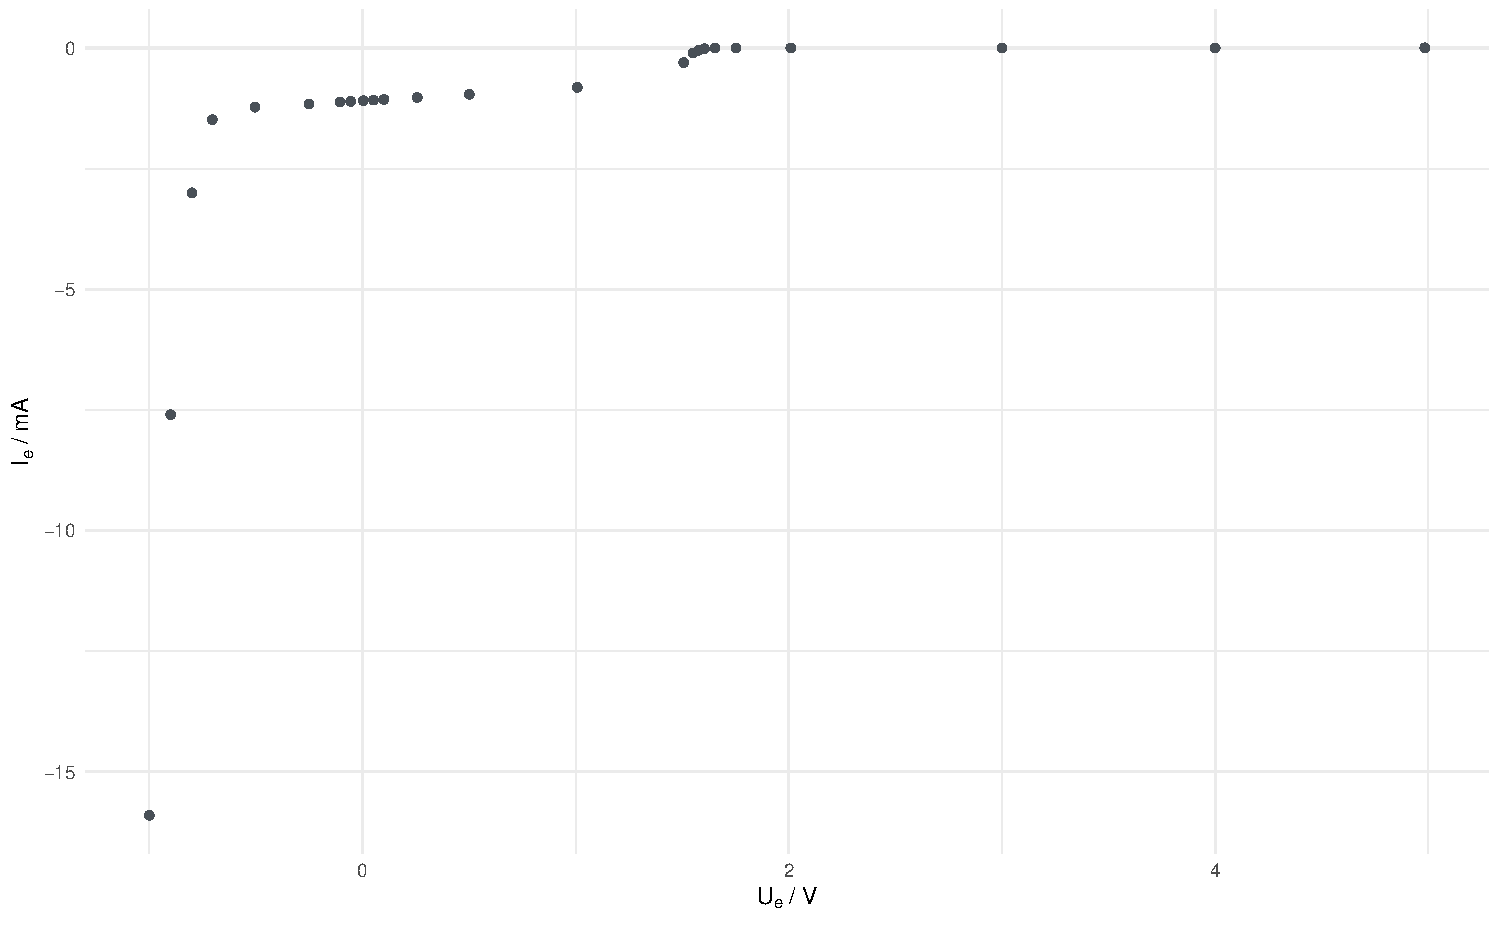
\includegraphics[width=\textwidth]{VERA/SN7400/SN7400_Eingangskennlinie}
  \end{center}
  \caption{gemessene Punkte der Eingangskennlinie des SN7400}
  \label{fig:7400_eingang}
\end{figure}